\chapter{Biblioteca Mathematical Components}
\label{cap:mathcomp}

Nos capítulos seguintes será usada uma série de itens disponíveis na biblioteca Mathematical Components e outros implementados com uso da biblioteca. Todavia é necessário, por parte do leitor, um conhecimento básico sobre essa biblioteca, e para isso, neste capítulo serão explicados elementos que foram considerados mais essenciais de acordo com o tema definido. Todo o conteúdo a seguir se baseia em \cite{assia_mahboubi_2022_7118596}.

Ademais, é importante ressaltar que, na apresentação dos conteúdos deste capítulo, se assume que o leitor possui um conhecimento básico sobre \textit{Coq}, e em caso contrário recomenda-se que o leitor acesse o material disponível em: \url{https://softwarefoundations.cis.upenn.edu/lf-current/index.html}

\section{Módulos}
A biblioteca Mathematical Components é divida em módulos, nos quais alguns são simplesmente a união de outros menores relacionados entre si. No site oficial da biblioteca\footnote{\url{https://math-comp.github.io/}} está disponível, além do livro utilizado como referência neste trabalho \cite{assia_mahboubi_2022_7118596}, um grafo
de tais módulos. A Figura \ref{fig:graph-mathcomp} apresenta uma parte desse grafo:

\begin{figure}[h]
    \centering
    \caption{Grafo do módulo ssreflect}
    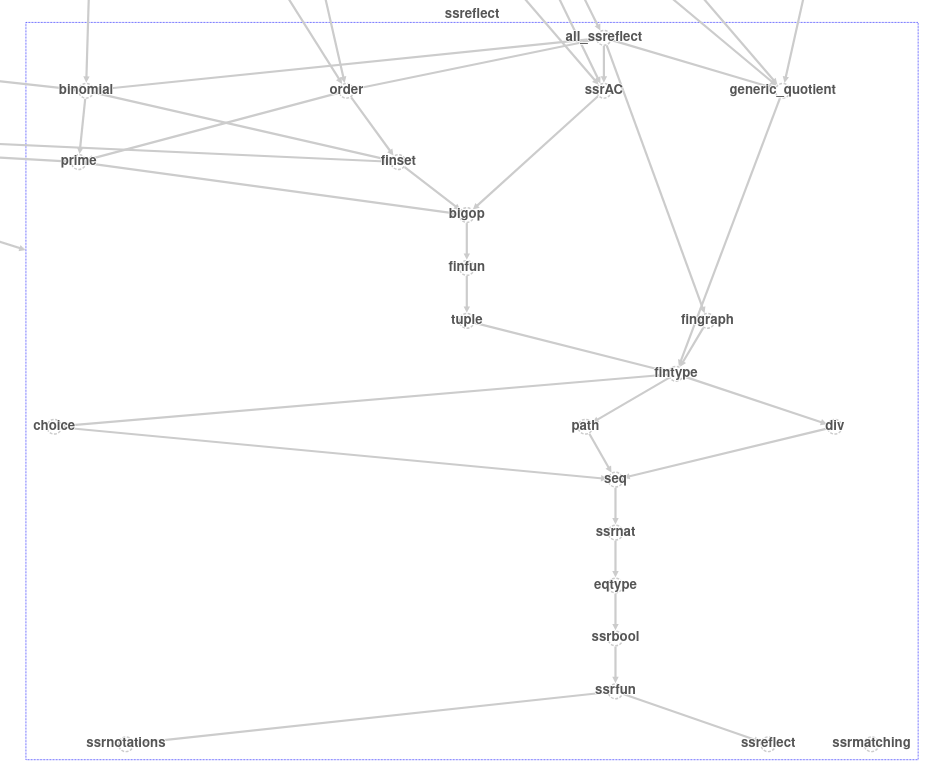
\includegraphics[width=0.6\textwidth]{Figuras/ssreflect.png}\\
    \footnotesize{Disponível em: <\url{https://math-comp.github.io/htmldoc_2_2_0/libgraph.html}>.
    Acesso em: 18 de maio de 2024.}
    \label{fig:graph-mathcomp}
\end{figure}

Os módulos principais para o desenvolvimento da prova sobre o algoritmo Tonelli-Shanks (com base no conteúdo de Teoria dos Números que sustenta a lógica do mesmo) são: \textit{all\_ssreflect} (que contém diversos outros módulos), \textit{ring\_quotient}, \textit{zmodp} e \textit{intdiv}.

\section{Igualdades}
Na maior parte dos teoremas das bibliotecas nativas de \textit{Coq}, usa-se uma definição indutiva de igualdade, que é por sua vez equivalente a igualdade de Leibniz (isto pode ser provado). Por sua vez, essa definição de igualdade é dada pela seguinte proposição indutiva (de acordo com a documentação\footnote{\url{https://coq.inria.fr/doc/V8.18.0/refman/proofs/writing-proofs/equality.html}} \cite{coqteam2022manual}):

\begin{lstlisting}[language = coq]
    Inductive eq {A : Type} (x : A) : A -> Prop := eq_refl : eq x x.
\end{lstlisting}

De maneira distinta, a biblioteca Mathematical Components, em suas definições e teoremas, utiliza com frequência predicados booleanos \cite{assia_mahboubi_2022_7118596}, que são basicamente funções cujo tipo de retorno é \lstinline[language = coq]!bool!, para então representar proposições da forma \lstinline[language = coq]$x = true$, onde \lstinline[language = coq]$x$ é uma expressão cujo retorno é do tipo \lstinline[language = coq]!bool!. Tais proposições são construídas pela função \lstinline[language = coq]$is_true$.No entanto, através do comando \lstinline[language = coq]$Coercion$ (que será explicado mais detalhadamente adiante neste documento) e por questões de legibilidade, tal função é omitida e o sistema de tipos de \textit{Coq} é capaz de inferir quando uma expressão deve ter tipo \lstinline[language = coq]$bool$ ou tipo \lstinline[language = coq]$Prop$ (e então há uma aplicação de \lstinline[language = coq]$is_true$ omitida). 

Semelhantes aos teoremas existentes para proposição comuns, estão disponíveis diversos teoremas para proposições geradas com o uso de \lstinline[language = coq]$is_true$, como por exemplo o lema \lstinline[language = coq]$contraLR$. Esse é uma versão da contraposição utilizando predicados booleanos (junto à função \lstinline[language = coq]$is_true$) e sua definição é dada por:
\begin{lstlisting}[language = coq]
        Lemma contraLR (c b : bool) : (~~ c -> ~~ b) -> b -> c.
\end{lstlisting}
onde \lstinline[language = coq]$~~$ é a operação de negação definida na biblioteca Mathematical Components.

Outra informação relevante ao se tratar do conteúdo da biblioteca é o tipo \lstinline[language = coq]$eqType$: para que seja construído qualquer habitante desse tipo é necessário um elemento \lstinline[language = coq]$T$ de tipo 
\lstinline[language = coq]$Type$, uma função \lstinline[language = coq]$eq_op$ de tipo \lstinline[language = coq]$T -> T -> bool$
e um elemento \lstinline[language = coq]$eqP$ cujo tipo é um teorema relacionando a igualdade de Leibniz com \lstinline[language = coq]$T$ e \lstinline[language = coq]$eq_op$. Este último possui, na biblioteca, uma notação de nome \lstinline[language = coq]$eq_axiom$, e sua descrição é:
\begin{lstlisting}[language = coq]
    Definition eq_axiom: forall (T : Type) (e : rel T), forall x x0 : T, 
            reflect (x = x0) (e x x0)
\end{lstlisting}
onde \lstinline[language = coq]$rel T$ é equivalente ao tipo \lstinline[language = coq]$T -> T -> bool$.

Portanto, para que um tipo \lstinline[language = coq]$A$
pertença ao primeiro campo mencionado, é necessário que se tenha uma prova da proposição \lstinline[language = coq]$eq_axiom A$, isto é, 
a definição \lstinline[language = coq]$eq_axiom$ com 
\lstinline[language = coq]$T$ igual a \lstinline[language = coq]$A$.
Tal teorema indica que a igualdade sobre \lstinline[language = coq]$A$
é decidível, o que fica claro pelo seguinte lema:

\begin{lstlisting}[language = coq]
    Lemma decP: forall (P : Prop) (b : bool), reflect P b -> decidable P
\end{lstlisting}

A utilização de um tipo como \lstinline[language = coq]$eqType$ facilita que se provem teoremas genéricos, no sentido de que servem para diferentes tipos (pertencentes a \lstinline[language = coq]$Type$) desde que estes possuam uma relação de equivalência decidível. Existem outros tipos semelhantes a \lstinline[language = coq]$eqType$, no sentido de que servem como interfaces. Em grande parte, esses são implementados por meio do açúcar sintático \lstinline[language = coq]$Record$, qual será explicado na sessão seguinte.

\section{Structures e Records} 
\label{section:structs-e-records}

\lstinline[language = coq]$Structure$ e \lstinline[language = coq]$Record$ são comandos sinônimos para geração de tipos indutivos que possuem somente um construtor e cujo os campos são dependentemente tipados, isto é, o tipo de cada campo pode depender dos valores de campos anteriores, assim como nas definições indutivas \cite{assia_mahboubi_2022_7118596}. A vantagem do uso desses comandos é que por meio desses são geradas automaticamente funções para extrair valores dos argumentos do construtor do tipo declarado.

Estes comandos são frequentemente utilizados na biblioteca Mathematical Components para definir interfaces (como o \lstinline[language = coq]$eqType$) e subtipos (ex.: tipo em que os habitantes são todos os números naturais menores que $8$). Para melhor entendimento do leitor, tem-se a seguir um exemplo semelhante ao tipo \lstinline[language = coq]$eqType$ definido na biblioteca, apresentado em \cite{assia_mahboubi_2022_7118596}:
\begin{lstlisting}[language = coq]
    Record eqType : Type := Pack
    {
        sort : Type;
        eq_op : sort -> sort -> bool;
        axiom : eq_axiom eq_op
    }.
\end{lstlisting}
Como explicado acima, essa declaração é equivalente a se fazer as seguintes declarações:
\begin{lstlisting}[language = coq]
        Inductive eqType : Type :=
            | Pack (sort : Type) (eq_op : sort -> sort -> bool) (axiom : eq_axiom eq_op).
            
        Definition sort (e : eqType) : Type :=
            match e with
            | Pack t _ _ => t
            end.
        Definition eq_op (e : eqType) : (sort e -> sort e -> bool) :=
            match e with
            | Pack _ f _ => f
            end.
        Definition axiom (e : eqType) : (eq_axiom (eq_op e)) :=
            | Pack _ _ a => a
            end.
\end{lstlisting}
Observe que o uso de tipos dependentes ocorre nos campos \lstinline[language = coq]{eq_op} e \lstinline[language = coq]{axiom}. No primeiro, o tipo do campo depende do valor do campo \lstinline[language = coq]{sort} e no segundo o tipo do campo depende do valor do campo \lstinline[language = coq]{eq_op} e portanto também do campo \lstinline[language = coq]{sort}.

\subsection{Comando Canonical} Assim como apresentado em \cite{assia_mahboubi_2022_7118596}, para instanciar um habitante de \lstinline[language = coq]$eqType$ com campo \lstinline[language = coq]$sort$ igual a \lstinline[language = coq]$nat$, deve-se provar o seguinte teorema:
\begin{lstlisting}[language = coq]
    Theorem axiom_nat: eq_axiom eqn.
\end{lstlisting}
onde \lstinline[language = coq]$eqn$ é uma operação de comparação booleana entre números naturais.
Tendo esta prova, podemos instanciar tal habitante
da seguinte forma:
\begin{lstlisting}[language = coq]
    Definition natEqtype := Pack nat eqn axiom_nat.
\end{lstlisting}
Note que, agora, pode-se comparar dois números naturais da seguinte maneira:
\begin{lstlisting}[language = coq]
    Compute (@eq_op natEqType 2 2).
\end{lstlisting}
o que nesse caso equivale a:
\begin{lstlisting}[language = coq]
    Compute (eqn 2 2).
\end{lstlisting}

Entretanto, o objetivo de criar o tipo \lstinline[language = coq]$eqType$ não é estabelecer essa possibilidade de computação para relações de comparação, mas sim construir definições, funções e provas genéricas para todos os tipos que pertencem ao campo \lstinline[language = coq]$sort$ de algum habitante de \lstinline[language = coq]$eqType$ e estabelecer \textit{overloading} de notações. Para exemplo de como alcançar este último objetivo, se define uma notação da seguinte forma:

\begin{lstlisting}[language = coq]
    Notation "x == y" := (@eq_op _ x y).
\end{lstlisting}
porém havendo apenas esta definição, caso executado o comando \lstinline[language = coq]$Check (3 == 2)$ tem-se um falha. Ao se executar:
\begin{lstlisting}[language = coq]
    Fail Check (3 == 2).
\end{lstlisting}
a seguinte mensagem é apresentada:
\begin{lstlisting}[language = coq-error]
    The command has indeed failed with message:
    The term "3" has type "nat" while it is 
    expected to have type "sort ?e"
\end{lstlisting}
Isto ocorre pois o \textit{Coq} não é capaz de inferir o argumento implícito\footnote{Note que o comando \lstinline[language = coq]$Fail Check (3 == 2)$ é equivalente a \lstinline[language = coq]$Fail Check (@eq_op _ 3 2)$.}  (\lstinline[language = coq]$_$).

Note que é mencionada uma variável \lstinline[language = coq]$?e$. Essa representa um elemento a ser inferido de modo que o tipo \lstinline[language = coq]$sort ?e$ seja igual ao tipo \lstinline[language = coq]$nat$. Como exposto em \cite{10.1007/978-3-642-39634-2_5} o algoritmo de inferência do \textit{Coq} não é capaz de descobrir o valor de tal variável por meio das regras de inferência que possui. Para resolver este problema 
o \textit{Coq} permite que se adicione regras de inferência de tipo por meio do comando \lstinline[language = coq]$Canonical$ (que recebe um construtor de algum \lstinline[language = coq]$Record$ ou \lstinline[language = coq]$Structure$ aplicado aos seus argumentos). Assim, resolver esse problema é possível por meio do seguinte código:
\begin{lstlisting}[language = coq]
    Canonical natEqType.
\end{lstlisting}
Com isto, de maneira semelhante ao exemplo exposto em \cite{10.1007/978-3-642-39634-2_5}, é adicionada a seguinte regra de inferência ao algoritmo presente em \textit{Coq}:

\begin{equation*}
        \inferrule 
        {
        \text{\lstinline[language = coq]!nat!} \sim 
        \text{\lstinline[language = coq]!sort natEqType!} 
        \\
        \; \text{\lstinline[language = coq]!?!} \text{\lstinline[language = coq]!e!} \; \sim
        \text{\lstinline[language = coq]!natEqType!} 
        }
        {\text{\lstinline[language = coq]!nat!} \sim \text{\lstinline[language = coq]!sort ?e!}}   
\end{equation*}
em que a notação $\sim$ representa uma chamada do algoritmo de unificação \cite{10.1007/978-3-642-39634-2_5} (que é o nome dado ao algoritmo de comparação de tipos chamado nas rotinas de inferência de tipos). Neste momento o leitor pode se perguntar como tal regra de inferência leva o algoritmo a chegar em um resultado final, e a resposta de acordo \cite{10.1007/978-3-642-39634-2_5} está em na existência de outras regras de inferência, como \textit{eq} e \textit{assign}:

\begin{equation*}
    \inferrule
    { }
    {
        \text{\lstinline[language = coq]!t!} \sim \text{\lstinline[language = coq]!t!}
    } \textit{eq}
    \hspace{20mm} % \text{&&}
    \inferrule
    { }
    {
        \text{\lstinline[language = coq]!?!\lstinline[language = coq]!x!} \sim \text{\lstinline[language = coq]!t!}
    } \textit{assign}
\end{equation*}
Retornando ao comando \lstinline[language = coq]$Check$, se agora esse for executado da mesma maneira feita anteriormente (porém sem o \lstinline[language = coq]$Fail$):
\begin{lstlisting}[language = coq]
    Check (3 == 2).
\end{lstlisting}
tem-se o seguinte resultado:
\begin{lstlisting}[language = coq-error]
    3 == 2
        : bool
\end{lstlisting}

Como mencionado previamente o tipo \lstinline[language = coq]$eqType$ serve para diversas generalizações. Para exemplo disso, adiante se apresenta a definição de uma comparação entre valores do tipo \lstinline[language = coq]$option$. Antes desse exemplo, vale aqui relembrar o leitor da definição deste tipo:
\begin{lstlisting}[language = coq]
    Inductive option (A : Type) : Type :=
        | None : option A
        | Some : A -> option A.
\end{lstlisting}
A função de comparação a ser declarada irá considerar que o argumento \lstinline[language = coq]$A$ pertence ao campo \lstinline[language = coq]$sort$ de algum habitante de \lstinline[language = coq]$eqType$. Tem-se então a definição dessa função:
\begin{lstlisting}[language = coq]
    Definition cmp_option (e : eqType) (o1 o2 : option (sort e)) :=
        match o1, o2 with
        | Some e1, Some e2 => op e e1 e2
        | None, Some _ => false
        | Some _, None => false
        | None, None => true
        end.
\end{lstlisting}
Agora, para criar um habitante de \lstinline[language = coq]$eqType$ para todo tipo da forma \lstinline[language = coq]$option A$ (note que para todo \lstinline[language = coq]$A$ diferente tem-se um tipo diferente) em que o tipo \lstinline[language = coq]$A$ segue o que foi considerado na função, deve-se provar o seguinte teorema:
\begin{lstlisting}[language = coq]
    Theorem axiom_option: 
        forall e : eqType, eq_axiom (cmp_option e).
\end{lstlisting}
que para facilidade de entendimento do leitor, pode ser escrito como:
\begin{lstlisting}[language = coq]
    Theorem axiom_option: 
        forall e : eqType, forall x y : option (sort e), reflect (x = y) (@cmp_option e x y).
\end{lstlisting}
Com esta prova pode-se construir a seguinte definição:
\begin{lstlisting}[language = coq]
    Definition optionEqType (e : eqType) := 
        Pack (option (sort e)) (cmp_option e) (axiom_option e).
\end{lstlisting}
Visto que ainda não foi executado o comando \lstinline[language = coq]$Canonical$ com esta definição, se executado o comando \lstinline[language = coq]$Check (Some 1 == Some 2)$, esse irá falhar, logo, ao se executar:
\begin{lstlisting}[language = coq]
    Fail Check (Some 1 == Some 2).
\end{lstlisting}
É apresentada a seguinte mensagem:
\begin{lstlisting}[language = coq-error]
    The command has indeed failed with message:
    The term "Some 1" has type "option nat" 
    while it is expected to have type "sort ?e".
\end{lstlisting}
Semelhante ao que foi feito anteriormente, para resolver este problema deve-se executar: 
\begin{lstlisting}[language = coq]
    Canonical optionEqType.
\end{lstlisting}
e com isso se adiciona a seguinte regra de inferência:
Semelhante ao que foi feito anteriormente, para resolver este problema deve-se executar: 
\begin{lstlisting}[language = coq]
    Canonical optionEqType.
\end{lstlisting}
e com isso se adiciona a seguinte regra de inferência:
\begin{equation*}
    \inferrule
    {
    \text{\lstinline[language = coq]!t!} \sim 
    \text{\lstinline[language = coq]!sort ?x!} 
    \\ 
    \text{\lstinline[language = coq]!?!\lstinline[language = coq]!e!} \sim
    \text{\lstinline[language = coq]!optionEqType ?x!} 
    }
    {
        \text{\lstinline[language = coq]!option t!} \sim \text{\lstinline[language = coq]!sort ?e!}
    }   
\end{equation*}
Assim note que no problema de inferência acima, ocorre a seguinte (sub)sequência de aplicação de regras de inferência para se determinar o valor de \lstinline[language = coq]$?e$:
\begin{equation*}
    \inferrule []
    {
        \inferrule []
        {
        \text{\lstinline[language = coq]!nat!} \sim 
        \text{\lstinline[language = coq]!sort natEqType!} 
        \\ 
        \text{\lstinline[language = coq]!?!\lstinline[language = coq]!x!} \sim
        \text{\lstinline[language = coq]!natEqType!} 
        }
        {\text{\lstinline[language = coq]!nat!} \sim \text{\lstinline[language = coq]!sort ?x!}} 
        % \lstinline[language = coq]!nat! \sim 
        % \lstinline[language = coq]!sort ?x! 
        \\ 
        \\
        \text{\lstinline[language = coq]!?!\lstinline[language = coq]!e!} \sim
        \text{\lstinline[language = coq]!optionEqType ?x!} 
    }
    {\text{\lstinline[language = coq]!option nat!} \sim \text{\lstinline[language = coq]!sort ?e!}}   
\end{equation*}
Agora, com o comando:
\begin{lstlisting}[language = coq]
    Check (Some 1 == Some 2).
\end{lstlisting}
tem-se a mensagem:
\begin{lstlisting}[language = coq-error]
    Some 1 == Some 2
        : bool
\end{lstlisting}

\subsection{Comando Coercion} \label{subsection:coercion}

Em provas manuais costuma-se utilizar notações iguais para operações sobre diferentes tipos. Como exemplo, há o uso do símbolo $+$ para operação de soma sobre os conjuntos númericos $\mathbb{N}$, $\mathbb{Z}$, $\mathbb{Q}$, $\mathbb{R}$ , como operador lógico \textit{ou} e também como operação binária qualquer que forma um monoide genérico. Nessa aplicação cotidiana de \textit{overloading} de notações, as informações sobre tipos são inferidas pelo cérebro humano conforme o contexto em que se encontram \cite{10.1007/978-3-642-39634-2_5}. 
Tomando isso em consideração e tendo em mente o conteúdo abordado na subseção anterior, pode-se dizer que o comando \lstinline[language = coq]$Canonical$ auxilia os usuários, tornando a escrita em \textit{Coq} mais semelhante a que se faz manualmente.

Outro mecanismo relacionado a tipos em \textit{Coq}, e que de certa forma serve para esse mesmo propósito, é provido pelo comando \lstinline[language = coq]$Coercion$. Como motivação para o uso deste, suponha a declaração em \textit{Coq} de um tipo que contenha todos os números naturais múltiplos de um número $n$. Utilizando \lstinline[language = coq]$Record$, temos então: 
\begin{lstlisting}[language = coq]
Record multiple (n : nat) : Type := Build
{       
    x : nat;
    axiom : (n %| x)        
}.
\end{lstlisting}
Observe que para construir um habitante deste tipo é dado um elemento \lstinline[language = coq]$n$ de tipo \lstinline[language = coq]$nat$ e é necessário um elemento \lstinline[language = coq]$x$ de mesmo tipo, e além disso, uma prova\footnote{Há de maneira implícita a aplicação da função \lstinline[language = coq]$is_true$ no tipo do campo \lstinline[language = coq]$axiom$, portanto o que foi declarado como tipo deste campo, isto é, \lstinline[language = coq]$n \%| x$, é equivalente a \lstinline[language = coq]$n \%| x = true$.} de que \lstinline[language = coq]$x$ é divisível por \lstinline[language = coq]$n$.
Agora, com tal declaração, visto que o objetivo da mesma é representar qualquer conjunto de números divisíveis por um determinado natural $n$, o usuário de \textit{Coq} provavelmente desejará que se possa escrever algo como:
\begin{lstlisting}[language = coq]
    forall (n : nat) (a : multiple n), a + 0 = a.
\end{lstlisting}
sem que o uso da operação de adição leve a um erro pela razão dessa possuir tipo \lstinline[language = coq]$nat -> nat -> nat$ enquanto o argumento \lstinline[language = coq]$a$ tem tipo \lstinline[language = coq]$multiple n$, quando a intenção do usuário é de que este último represente um número natural. Se for utilizado o comando \lstinline[language = coq]$Check$ na proposição acima:
\begin{lstlisting}[language = coq]
    Fail Check (forall (n : nat) (a : multiple n), a + 0 = a).
\end{lstlisting}
tem-se a mensagem:
\begin{lstlisting}[language = coq-error]
    The command has indeed failed with message:
    In environment
    n : nat
    a : multiple n
    The term "a" has type "multiple n" while it is
    expected to have type "nat".
\end{lstlisting}
Buscando solucionar este tipo de problema, sem que tenha que se escrever:
\begin{lstlisting}[language = coq]
    forall (n : nat) (a : multiple n), (x n a) + 0 = (x n a).
\end{lstlisting}
o que por sua vez não geraria erro algum pois \lstinline[language = coq]$(x n a)$ tem tipo \lstinline[language = coq]$nat$\footnote{Lembre-se que \lstinline[language = coq]$x$, no contexto externo a declaração do seu respectivo \lstinline[language = coq]$Record$, é uma função que extrai o campo \lstinline[language = coq]$x$ de um elemento do tipo \lstinline[language = coq]$multiple n$ (para qualquer \lstinline[language = coq]$n$) e não o valor do campo em si. Portanto a seguinte definção poderia ser dada simplesmente como \lstinline[language = coq]$x$.}, defini-se uma função que retira o campo \lstinline[language = coq]$x$ de um elemento como \lstinline[language = coq]$a$:
\begin{lstlisting}[language = coq]
    Definition multiple_nat (n : nat) (e : multiple n) : nat :=
        let t := (x n e) in t.
\end{lstlisting}
e agora, para que o \textit{Coq} aplique esta função de maneira implícita, de modo a evitar erros de tipo, usa-se o comando \lstinline[language = coq]$Coercion$ da seguinte maneira:
\begin{lstlisting}[language = coq]
    Coercion multiple_nat : multiple >-> nat.
\end{lstlisting}
Agora, realizando o comando \lstinline[language = coq]$Check$ como anteriormente:
\begin{lstlisting}[language = coq]
    Check (forall n (a : multiple n), a + 0 = 0).
\end{lstlisting}
é gerada a mensagem:
\begin{lstlisting}[language = coq-error]
    forall (n : nat) (a : multiple n), a + 0 = 0
        : Prop
\end{lstlisting}

\subsection{Exemplo de Implementação de grupos}
\label{sub:grupos}

Um uso semelhante do mecanismo \textit{coercion}, junto ao \textit{canonical}, pode ser proposto com um tipo que representa grupos. Um grupo é uma estrutura algébrica dada por $(G, \otimes)$ onde:
\begin{enumerate}
    \item $\otimes$ é uma operação binária sobre $G$, isto é, $\otimes$ é uma função tal que $\otimes : (G \times G) \rightarrow G$.
    \item $\otimes$ é associativa, ou seja, $\forall a, b \in G, (a \otimes b) \otimes c = a \otimes (b \otimes c)$.
    \item Existe um elemento neutro $e$, o que significa: $\exists e \in G (\forall a \in G, e \otimes a = a \otimes e = a)$. 
    \item Para todo elemento em $G$ existe um elemento inverso, isto é, \\
    $\forall x \in G (\exists \;\overline{x} \in G, x \;\otimes\; \overline{x} = \overline{x} \;\otimes\; x = e)$
\end{enumerate}
Em \textit{Coq} um grupo pode ser representado pelo seguinte \lstinline[language = coq]$Record$:
\begin{lstlisting}[language = coq]
    Record Group : Type := group 
    {
        sort :> Type;
        bin_op : sort -> sort -> sort;
        associative_axiom : associative bin_op;
        e : sort;
        neutral_left : left_id e bin_op;
        neutral_right : right_id e bin_op;
        inverse_left : \forall x : sort, \exists y : sort, bin_op y x = e; 
        inverse_right : \forall x : sort, \exists y : sort, bin_op x y = e 
    }.
\end{lstlisting}
Observe que, diferente dos exemplos anteriores, o campo \lstinline[language = coq]$sort$ é seguido de \lstinline[language = coq]$:>$. Esse operador além de atribuir o tipo de \lstinline[language = coq]$sort$ como \lstinline[language = coq]$Type$
define a função \lstinline[language = coq]$sort$ como uma \textit{coercion} para todo habitante do tipo \lstinline[language = coq]$Group$. Assim, suponha a definição do seguinte habitante:
\begin{lstlisting}[language = coq]
    Definition int_group := 
        Group int addz addzA 0 add0z addz0 inverse_left_int inverse_right_int.
\end{lstlisting}
Esse habitante tem como campo \lstinline[language = coq]$sort$ o tipo \lstinline[language = coq]$int$ (que representa os números inteiros) e devido a \textit{coercion}, se for feita uma declaração com uma variável de tipo \lstinline[language = coq]$int_group$ em que se aplica uma função de tipo \lstinline[language = coq]$int -> int$ sobre esta variável, o \textit{Coq} irá automaticamente tratar a variável como tendo tipo \lstinline[language = coq]$int$ (ou mais especificamente, irá tratá-la como se fosse o valor de seu campo \lstinline[language = coq]$sort$, aplicando de maneira implícita a função \lstinline[language = coq]$sort$ sobre a mesma).

Para fins de demonstrar uma implentação completa de grupos em \textit{Coq}, define-se agora uma notação para as operações binárias e uma para os elementos neutros que formam grupos quaisquer, da seguinte forma:
\begin{lstlisting}[language = coq]
    Notation "x \otimes y" := (@bin_op _ x y) (at level 10).
    Notation "0" := (@e _).
\end{lstlisting}
Usa-se então o comando \lstinline[language = coq]$Canonical$ para que o \textit{Coq} seja capaz de inferir os argumentos implícitos presentes nas descrições destas notações (para o caso de \lstinline[language = coq]$x$ e  \lstinline[language = coq]$y$ possuirem tipo  \lstinline[language = coq]$int$):
\begin{lstlisting}[language = coq]
    Canonical int_group.
\end{lstlisting}
Com este conjunto de configurações passa a ser mais fácil a escrita e leitura de declarações relacionadas a grupos. Assim, torna-se então possível a formalização compacta de teoremas genéricos sobre quaisquer tipos presentes no campo \lstinline[language = coq]$sort$ de algum habitante de \lstinline[language = coq]$group$. Como exemplo, tem-se o seguinte teorema e sua respectiva prova:
\begin{lstlisting}[language = coq]
    Theorem exemplo_sobre_grupos: 
        \forall G : group, \forall a b : G, (a \otimes b) \otimes 0 = (a \otimes 0) \otimes b.
    Proof.
        intros. rewrite (neutral_right G). rewrite (neutral_right G).
        reflexivity. 
    Qed.
\end{lstlisting}
Como este teorema serve para qualquer grupo \lstinline[language = coq]$G$, esse pode então ser usado na seguinte prova:
\begin{lstlisting}[language = coq]
    Theorem exemplo_sobre_int:
        \forall a b : int, (a + b) + 0 = (a + 0) + b.
    Proof.
        apply exemplo_sobre_grupos.
    Qed.
\end{lstlisting}
Tal prova exemplifica como o uso dos mecanismos em \textit{Coq}, que foram apresentados neste capítulo, podem ser utilizados para que seja mais fácil trabalhar com um vasta quantidade de tipos que apresentam propriedades em comum (como é o caso dos grupos).

\subsection{Mantendo Informações de um Record ou Structure}

Em meio as provas que envolvem tipos de \lstinline[language = coq]$Record$ ou \lstinline[language = coq]$Structure$, o usuário de \textit{Coq} pode se deparar com situações em que, ao se aplicar uma determinada função sobre uma variável relacionada a um desses comandos, que portanto apresenta um determinado conjunto de propriedades, o resultado da computação dessa função irá retornar um dado do tipo definido pela \textit{coercion}. Em algumas dessas ocasiões, no entanto, a função aplicada retornará um dado com o qual se poderia construir uma nova variável do mesmo tipo de \lstinline[language = coq]$Record$ (ou \lstinline[language = coq]$Structure$) do elemento do qual o argumento da função foi extraído. Manter o tipo do resultado como o mesmo \lstinline[language = coq]$Record$ ou \lstinline[language = coq]$Structure$ pode ser útil em algumas provas, e fazer isso é possível através do comando \lstinline[language = coq]$Canonical$. A exemplo disso, retomando ao tipo \lstinline[language = coq]$multiple$, note que é possível provar os dois seguintes teoremas:
\begin{lstlisting}[language = coq]
    Theorem exemplo_multiple_axiom {n} :
        \forall (a : multiple n), n %| a.

    Theorem exemplo_aplicacao_f_mul {n} :
        \forall (f : nat -> nat) (a : multiple n), n %| (f a) * n.
\end{lstlisting}
onde \lstinline[language = coq]$%%$ é a operação de resto da divisão. Agora, imagine que se queira provar o seguinte:
\begin{lstlisting}[language = coq]
    Example exemplo_a_provar {n} :
        \forall (a : multiple n), (n %| ((fun x => x + 2) a) * n).
\end{lstlisting}
Note que, se tratando \lstinline[language = coq]!multiple n! como um conjunto de números naturais (apesar desse não ser precisamente isso) faria sentido poder utilizar o teorema \lstinline[language = coq]!exemplo_multiple_axiom! para reescrever o lado esquerdo da equação como \lstinline[language = coq]!true! (o operador  \lstinline[language = coq]!%|! tem tipo \lstinline[language = coq]!nat -> nat -> bool! portanto há uma \textit{coercion} \lstinline[language = coq]!is_true! na declaração do exemplo), ao invés de ter que utilizar um teorema mais específico como \lstinline[language = coq]!exemplo_aplicacao_f_mul!. Dado que se trata de uma aplicação de função em que após a aplicação o resultado é multiplicado por \lstinline[language = coq]!n!, é óbvio que o resultado da expressão:
\begin{lstlisting}[language = coq]
    (((fun x => x + 2) a) * n)
\end{lstlisting} 
é divisível por \lstinline[language = coq]!n!. Entretanto, a reescrita desejada não é possível pois ocorre um problema de unificação ao tentar se usar a tática \lstinline[language = coq]!rewrite exemplo_multiple_axiom!. Para obter-se uma melhor noção sobre este problema é possível utilizar o seguinte código fornecido por \cite{assia_mahboubi_2022_7118596} (sobre o qual a explicação de seu funcionamento vai além do escopo do presente trabalho):
\begin{lstlisting}[language = coq]
    Notation "X (*...*)" :=
    (let x := X in let y := _ in x) (at level 100, format "X  (*...*)").

    Notation "[LHS 'of' equation ]" := 
        (let LHS := _ in 
            let _infer_LHS := equation : LHS = _ in LHS) (at level 4).

    Notation "[unify X 'with' Y ]" := 
        (let unification := erefl _ : X = Y in True).
\end{lstlisting} 
Com isso, pode-se executar o seguinte comando:
\begin{lstlisting}[language = coq]
    Fail Check (forall n (a : multiple n) (f : nat -> nat),
        let LHS := [LHS of exemplo_multiple_axiom _] in
        let RDX := (n %| (f a) * n) in
        [unify LHS with RDX]).
\end{lstlisting}
Este comando irá apresentar uma mensagem de confirmação da falha, que em parte, apresenta o seguinte conteúdo:
\begin{lstlisting}[language = coq-error]
    The command has indeed failed with message:
    In environment
    n :
    nat
    a : multiple n
    f : nat -> nat
    LHS := [LHS of exemplo_multiple_axiom ?a] : bool
    RDX := n %| f (x n a) * n : bool
    The term "erefl LHS" has type "LHS = LHS"
    while it is expected to have type "LHS = RDX"
\end{lstlisting} 
Com isto, pode-se verificar que o problema de unificação encontrado é descobrir qual o valor da variável \lstinline[language = coq]!?a!. De modo mais específico, o problema está em encontrar um valor que torne equivalentes as seguintes expressões:
\begin{lstlisting}[language = coq]
    n %| (x n ?a)
\end{lstlisting} 
e
\begin{lstlisting}[language = coq]
    n %| ((f (x n a)) * n)
\end{lstlisting}
 Para resolver este problema % e então simular tal tratamento de \lstinline[language = coq]!smaller n! como um conjunto (para este caso em específico) em \textit{Coq}, 
 usa-se o comando \lstinline[language = coq]!Canonical! junto ao teorema\\ 
 \lstinline[language = coq]!exemplo_aplicacao_f_mul!, através do seguinte código:
\begin{lstlisting}[language = coq]
    Canonical f_mul_multiple {n : nat} (f : nat -> nat) (a : multiple n) := 
        (@Build n ((f a) * n) (@exemplo_aplicacao_f_mul n f a)).
\end{lstlisting} 
    Retornando então a prova de motivação para introdução ao problema discutido\\
    (\lstinline[language = coq]!exemplo_a_provar!) e utilizando a tática:
\begin{lstlisting}[language = coq]
    intros. simpl.
\end{lstlisting} 
O \textit{goal} da prova se torna:
\begin{lstlisting}[language = coq]
    n %| (a + 2) * n
\end{lstlisting}
Agora, para que se possa aplicar novamente a tática \lstinline[language = coq]!rewrite exemplo_smaller_axiom!, é necessário deixar o \textit{goal} escrito de modo que a expressão mais interna:
\begin{lstlisting}[language = coq]
    (a + 2)
\end{lstlisting}
fique na forma de uma função aplicada sobre um elemento múltiplo de \lstinline[language = coq]!n!.
Isso é necessário para que o \textit{Coq} possa inferir um elemento do tipo \lstinline[language = coq]!multiple n! dado pela definição \lstinline[language = coq]!f_mul_multiple!, permitindo assim o uso do teorema \lstinline[language = coq]!exemplo_multiple_axiom!. Como \lstinline[language = coq]!2! é de tipo \lstinline[language = coq]!nat!, o \textit{Coq} não consegue construir um habitante do tipo \lstinline[language = coq]!multiple n! que resolva o problema de unificação. O que se pode então fazer é inverter a ordem da função de soma, realizando a tática \lstinline[language = coq]!rewrite addnC!, em que \lstinline[language = coq]!addnC! é um teorema de comutativa da soma. Assim, o \textit{goal} resultante será:
\begin{lstlisting}[language = coq]
    n %| ((2 + a) * n)
\end{lstlisting}
Agora, utilizando novamente a tática \lstinline[language = coq]!rewrite exemplo_multiple_axiom!, tem-se:
\begin{lstlisting}[language = coq]
    true
\end{lstlisting}
Com isso a prova pode ser finalizada com o uso de 
\lstinline[language = coq]!reflexivity!.